\section{時間応答に基づくパラメータ同定}
\subsection{パラメータ同定とは?}

制御対象の物理パラメータの値は,はかりやメジャーなどの測定器で直接はかることができるとは限らない.
制御対象の物理パラメータの値がわからないと,制御対象の数学モデルに基づいたコントローラ設計やシミュレーションを行うことができない.
そこで,測定器で直接はかることができない物理パラメータを定めるため,制御対象に様々な信号を加え,このときの出力応答から物理パラメータの値を定める必要がある.このことを\textbf{パラメータ同定}と呼ぶ.

本実験装置の場合,\ref{sec:2_1} 節で述べたように,$v_x(t)$,$v_y(t)$ から $\theta_x(t)$,$\theta_y(t)$ への伝達関数 $G_x(s)$,$G_y(s)$ は
\begin{equation}
\left\{
\begin{aligned}
G_x(s) &= \frac{b_x}{s(s + a_x)}, \quad a_x = \frac{c_x}{J_x}, \quad b_x = \frac{k_{fx}}{J_x}, \\
G_y(s) &= \frac{b_y}{s(s + a_y)}, \quad a_y = \frac{c_y}{J_y}, \quad b_y = \frac{k_{fy}}{J_y}
\end{aligned}
\right.
\label{eq:gx_gy_transfer}
\end{equation}

であるから,$a_x$,$b_x$,$a_y$,$b_y$ の値を実験により定めることになる.
パラメータ同定を行う方法には,ステップ応答などの時間応答に基づく方法と周波数応答に基づく方法があるが,ここでは,時間応答に基づく方法を用いる.

\subsection{パラメータ同定の手順}

\paragraph{Pコントローラ}

\begin{equation}
    v_x(t) = k_{Px}(\theta_x^{\mathrm{ref}}(t) - \theta_x(t)) \tag{4.2}
\end{equation}

によりリンク1の関節角 $\theta_x(t)$ を制御したとき,2軸ロボットの数学モデル(式(2.4))と仮定すると,$\theta_x^{\mathrm{ref}}(s)$ から $\theta_x(s)$ への伝達関数は2次遅れ系

\begin{align}
    T_x(s) = \frac{G_x(s)k_{Px}}{1 + G_x(s)k_{Px}} = \frac{b_x k_{Px}}{s^2 + a_x s + b_x k_{Px}} = \frac{\omega_{nx}^2}{s^2 + 2 \zeta_x \omega_{nx} s + \omega_{nx}^2} \tag{4.3}
\end{align}

\[
\left\{
\begin{aligned}
    &\text{固有角周波数:} && \omega_{nx} = \sqrt{b_x k_{Px}} \\
    &\text{減衰係数:} && \zeta_x = \frac{a_x}{2 \omega_{nx}} = \frac{a_x}{2\sqrt{b_x k_{Px}}}
\end{aligned}
\right. \tag{4.4}
\]

となる.

(4.4)式から明らかなように,比例ゲイン $k_{Px}$ を大きくすると $\zeta_x$ は零に近づくため,ステップ応答はオーバーシュートが生じ,振動的になっていく.そこで,ある程度大きな比例ゲイン $k_{Px}$ を設定し,
目標値を

\begin{equation}
    \theta_x^{\mathrm{ref}}(t) = 
    \begin{cases}
        0 & (t < 0) \\
        \theta_{dx} & (t \geq 0)
    \end{cases} \tag{4.5}
\end{equation}

としたステップ応答にオーバシュートを生じさせると,最大ピーク値 $\max \theta_x$ と行き過ぎ時間 $t_{px}$ は以下のようになる.

\begin{equation}
    \left\{
    \begin{aligned}
        \max \theta_x &= \theta_{dx} \left(1 + \exp\left(-\frac{\gamma_x \pi}{\delta_x} \right) \right) \\
        t_{px} &= \frac{\pi}{\delta_x}
    \end{aligned}
    \right. \tag{4.6}
\end{equation}


ただし,

\begin{equation}
    \delta_x = \zeta_x \omega_{nx}, \quad \gamma_x = \omega_{nx} \sqrt{1 - \zeta_x^2} \tag{4.7}
\end{equation}

以上のことから,未知パラメータ $a_x$,$b_x$ の同定手順は以下のようになる.

パラメータ同定の手順
    \begin{enumerate}
        \item ある程度大きい比例ゲイン $k_{Px}$ を設定し,Pコントローラによるリンク1の角度制御を行う.ただし,$\theta_{dx}$ はあまり大きく設定しないようにする.たとえば,$k_{Px} = 20$,$\theta_{dx} = 0.2$ とする.
    
        \item 1) で設定した $k_{Px}$,$\theta_{dx}$ を用いて実機実験を行い,$\theta_x(t)$ をデータ列 $\theta_x^{\mathrm{data}}$ として取得する.
    
        \item 2) で取得したデータ $\theta_x^{\mathrm{data}}$ の最大値 $\max \theta_x^{\mathrm{data}}$ とそのときの時間 $t_{px}^{\mathrm{data}}$ を求める.
    
        \item $\gamma_x$,$\delta_x$ の同定値を以下の式により導出する:
        \[
            \gamma_x^{\mathrm{data}} = -\frac{1}{t_{px}^{\mathrm{data}}} \log_e \left( \frac{\max \theta_x^{\mathrm{data}}}{\theta_{dx}} - 1 \right) \tag{4.8}
        \]
        \[
            \delta_x^{\mathrm{data}} = \frac{\pi}{t_{px}^{\mathrm{data}}} \tag{4.9}
        \]
    
        \item 固有角周波数 $\omega_{nx}$,減衰係数 $\zeta_x$ の同定値を以下で定める:
        \[
            \omega_{nx}^{\mathrm{data}} = \sqrt{ (\gamma_x^{\mathrm{data}})^2 + (\delta_x^{\mathrm{data}})^2 } \tag{4.10}
        \]
        \[
            \zeta_x^{\mathrm{data}} = \frac{\gamma_x^{\mathrm{data}}}{\omega_{nx}^{\mathrm{data}}} \tag{4.11}
        \]
    
        \item $a_x$,$b_x$ の同定値 $a_x^{\mathrm{data}}$,$b_x^{\mathrm{data}}$ を次式により定める:
        \[
            a_x^{\mathrm{data}} = 2 \zeta_x^{\mathrm{data}} \omega_{nx}^{\mathrm{data}} \tag{4.12}
        \]
        \[
            b_x^{\mathrm{data}} = \frac{(\omega_{nx}^{\mathrm{data}})^2}{k_{Px}} \tag{4.13}
        \]
    \end{enumerate}
    
なお,未知パラメータ $a_y$,$b_y$ の同定手順は $a_x$,$b_x$ の同定手順と同様なので,ここでは省略する.

\noindent
\textbf{ステップ 1}:
まず,MATLAB/Simulink を起動し,以下の M ファイル ``\texttt{idarm.m}'' と
実機実験モデル ``\texttt{ex\_P.slx}'' を作成し,フォルダ \texttt{\textyen ID} に保存する.

\begin{figure}[htbp]
    \centering
    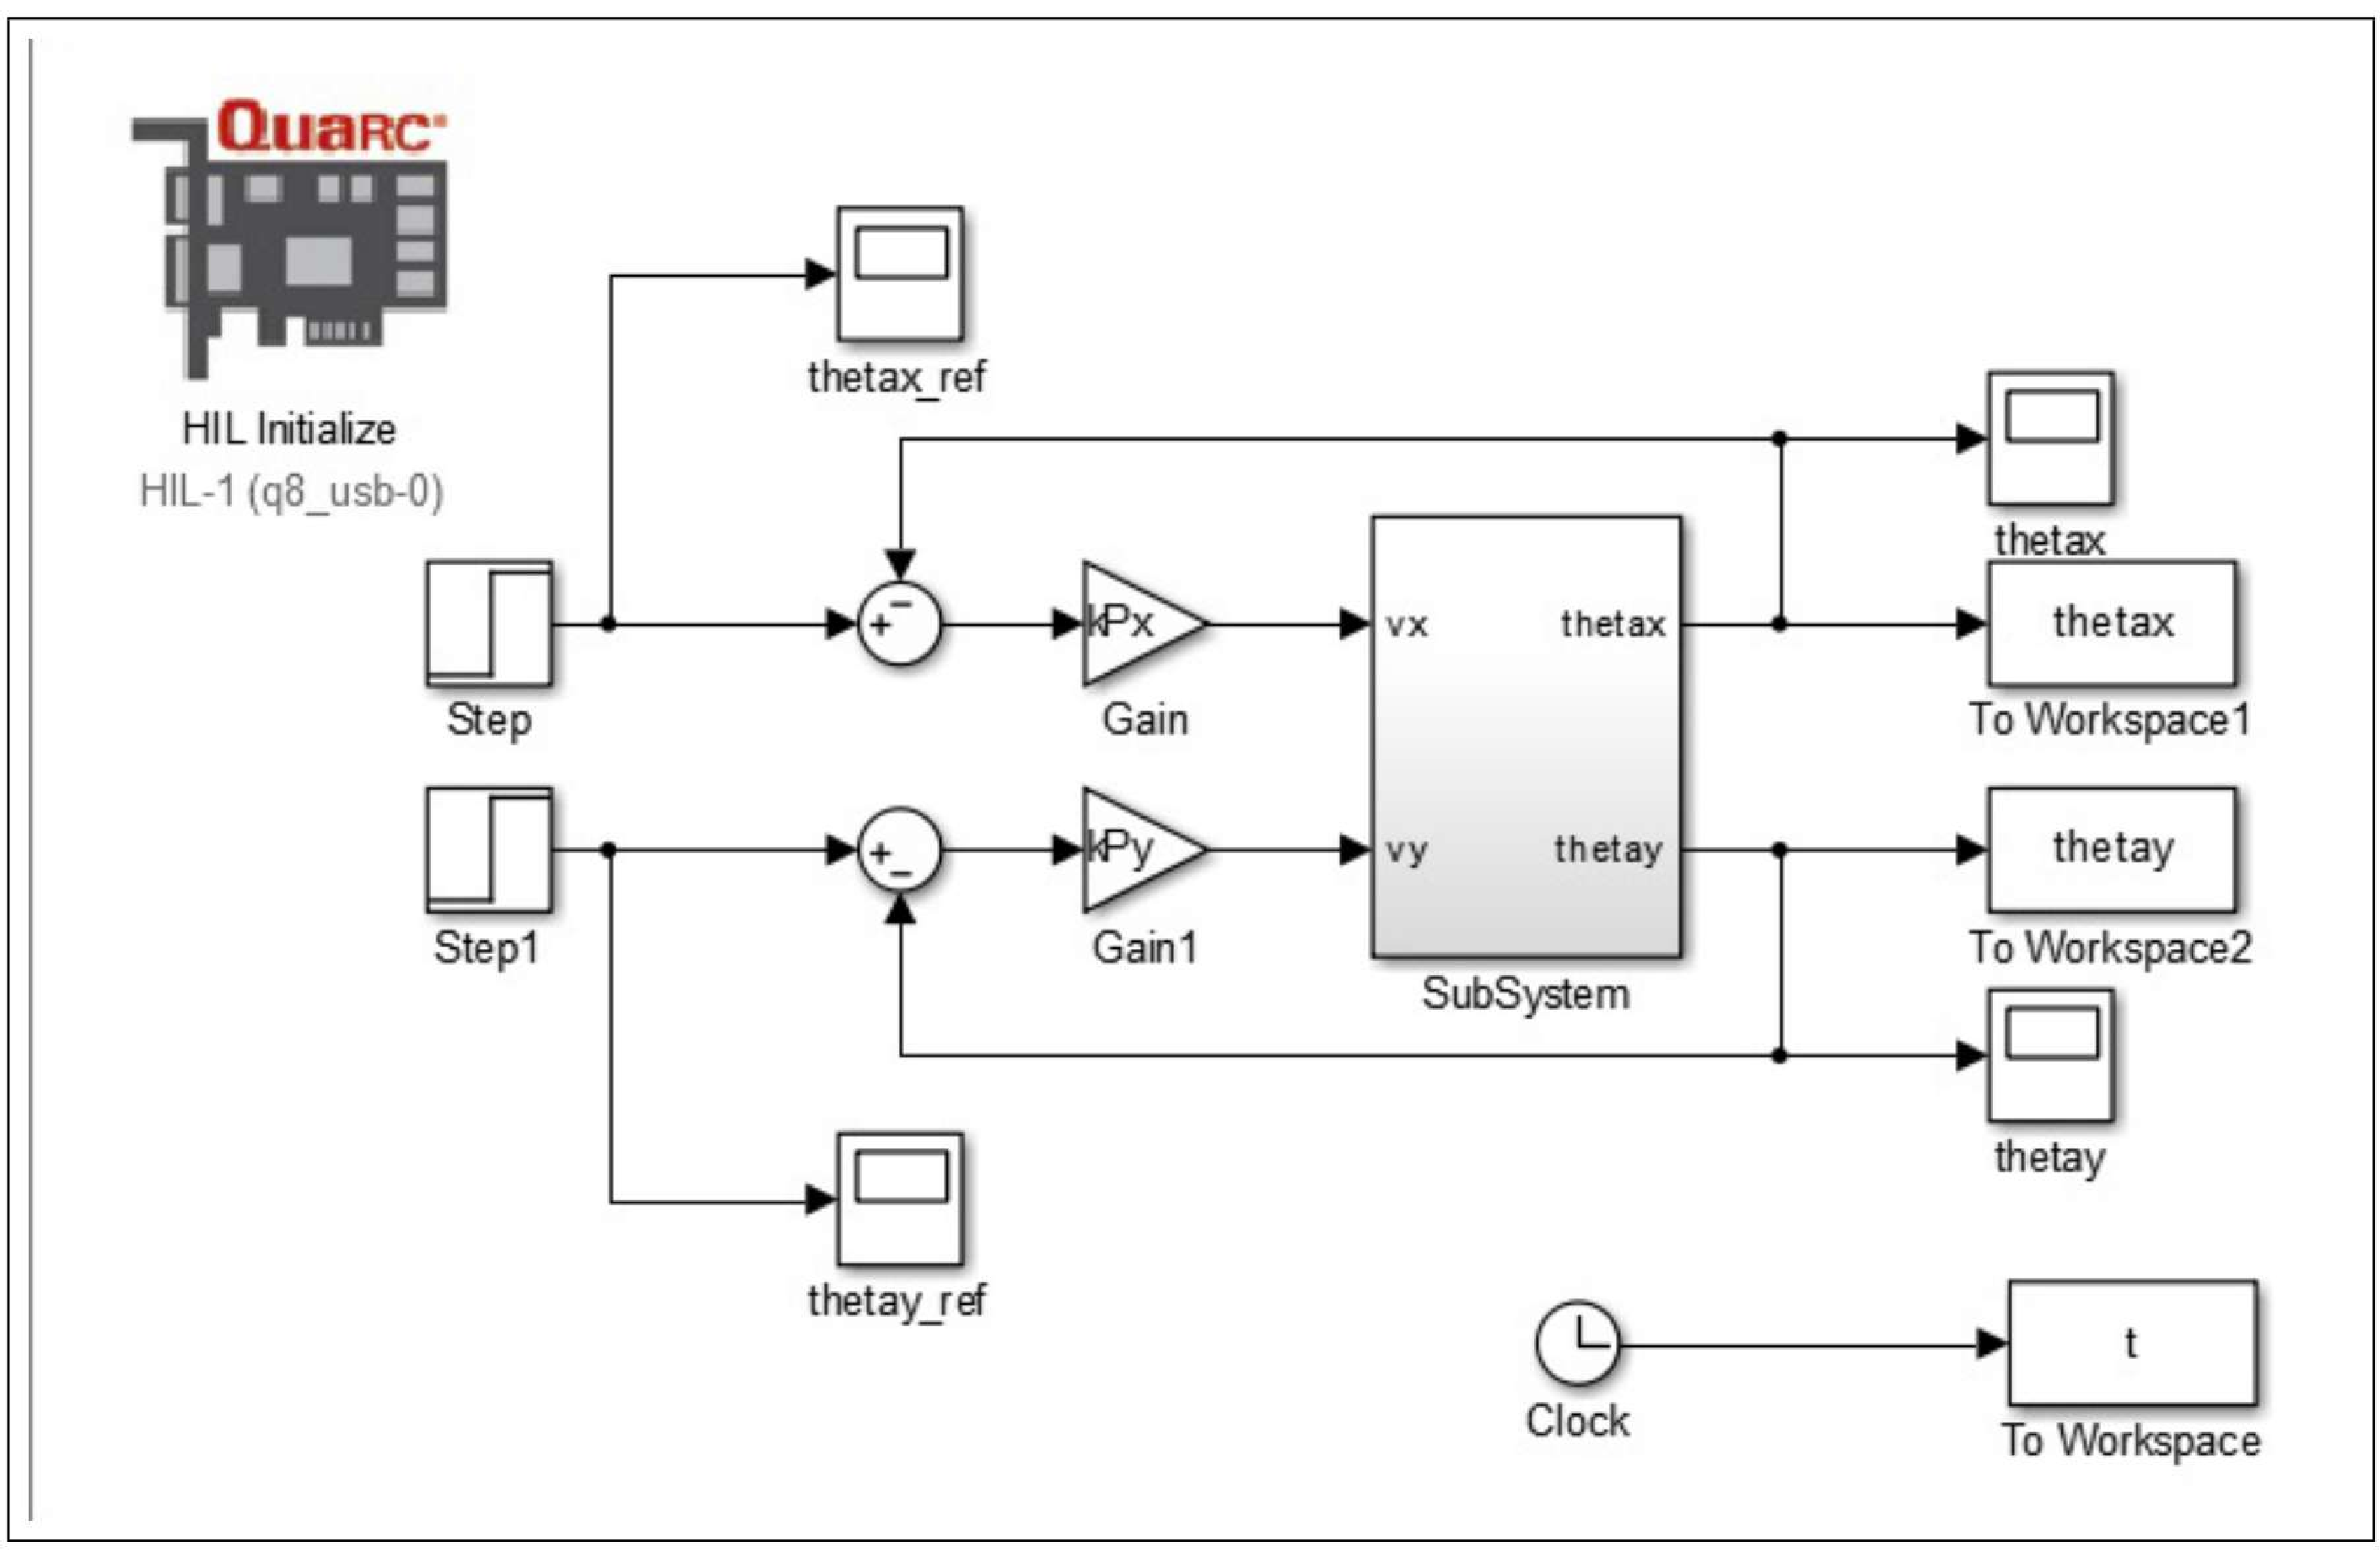
\includegraphics[width=0.9\linewidth]{figure/step2_model.pdf}
    \caption{P 制御の Simulink モデル(実機実験モデル ``\texttt{ex\_P.slx}'')}
    \label{fig:simulink_model_p}
\end{figure}

\vspace{1em}
\noindent
\textbf{ステップ 2}:
ステップ 1 の \texttt{\textyen ID} をカレントフォルダとして,実機実験モデル ``\texttt{ex\_P.slx}'' をコンパイルする.

\vspace{1em}
\noindent
\textbf{ステップ 2}:
ステップ1の \texttt{\textyen ID} をカレントフォルダとして,実機実験モデル ``\texttt{ex\_P.slx}'' をコンパイルする.

\vspace{1em}
\noindent
\textbf{ステップ 3}:
モータ軸の角度 $\theta_x(t)$ と $\theta_y(t)$ が $0$~[rad] となるように P 制御する.
実機実験モデル ``\texttt{ex\_P.slx}'' のブロック ``Step'',``Step1'' をダブルクリックし,

\[
\begin{array}{ll}
\text{Step}~(\theta_x^{\mathrm{ref}}(t))\!: &
\left\{
\begin{array}{l}
\text{ステップ時間: } 0 \\
\text{初期値: } 0 \\
\text{最終値: } 0 \\
\text{サンプル時間: } 0
\end{array}
\right., \quad
\text{Step1}~(\theta_y^{\mathrm{ref}}(t))\!: 
\left\{
\begin{array}{l}
\text{ステップ時間: } 0 \\
\text{初期値: } 0 \\
\text{最終値: } 0 \\
\text{サンプル時間: } 0
\end{array}
\right.
\end{array}
\]

のように変更して,モータ軸の目標角度 $\theta_x^{\mathrm{ref}}(t)$,$\theta_y^{\mathrm{ref}}(t)$ を設定する.
ターゲットに接続し,実行してアーム角度が $0$ になっていることを確認する.

\vspace{1em}
\noindent
\textbf{ステップ 4}:
実機実験モデル ``\texttt{ex\_P.slx}'' のブロック ``Step'',``Step1'' をダブルクリックし,

\[
\begin{array}{ll}
\text{Step}~(\theta_x^{\mathrm{ref}}(t))\!: &
\left\{
\begin{array}{l}
\text{ステップ時間: } 0 \\
\text{初期値: } 0 \\
\text{最終値: } 0.2 \\
\text{サンプル時間: } 0
\end{array}
\right., \quad
\text{Step1}~(\theta_y^{\mathrm{ref}}(t))\!: 
\left\{
\begin{array}{l}
\text{ステップ時間: } 0 \\
\text{初期値: } 0 \\
\text{最終値: } 0.2 \\
\text{サンプル時間: } 0
\end{array}
\right.
\end{array}
\]

のように変更して,モータ軸の目標角度 $\theta_x^{\mathrm{ref}}(t)$,$\theta_y^{\mathrm{ref}}(t)$ を設定する.
\vspace{1em}
\noindent
\textbf{ステップ 5}: MATLAB Command Window で M ファイル ``\texttt{idarm.m}'' を実行すると,

\begin{tabbing}
\hspace{1cm}\=\kill
\> \texttt{>> idarm} \\
\> \texttt{ax = 40.9262} \hspace{6cm} \texttt{a\_x = 40.9262} \\
\> \texttt{bx = 76.7858} \hspace{6cm} \texttt{b\_x = 76.7858} \\
\> \texttt{ay = 42.1695} \hspace{6cm} \texttt{a\_y = 42.1695} \\
\> \texttt{by = 75.7744} \hspace{6cm} \texttt{b\_y = 75.7744}
\end{tabbing}

\vspace{1em}
\noindent
ようになり,パラメータの同定値が計算される.また,図~\ref{fig:step_response2} に示すグラフが表示される.なお,図~\ref{fig:step_response} における実線は実験データ,破線は同定された値を用いたシミュレーションデータのプロットである.また,$a_x$,$b_x$,$a_y$,$b_y$ は \texttt{armpara.mat} に保存されている.

\begin{figure}[htbp]
    \centering
    \begin{subfigure}[b]{0.45\linewidth}
        \centering
        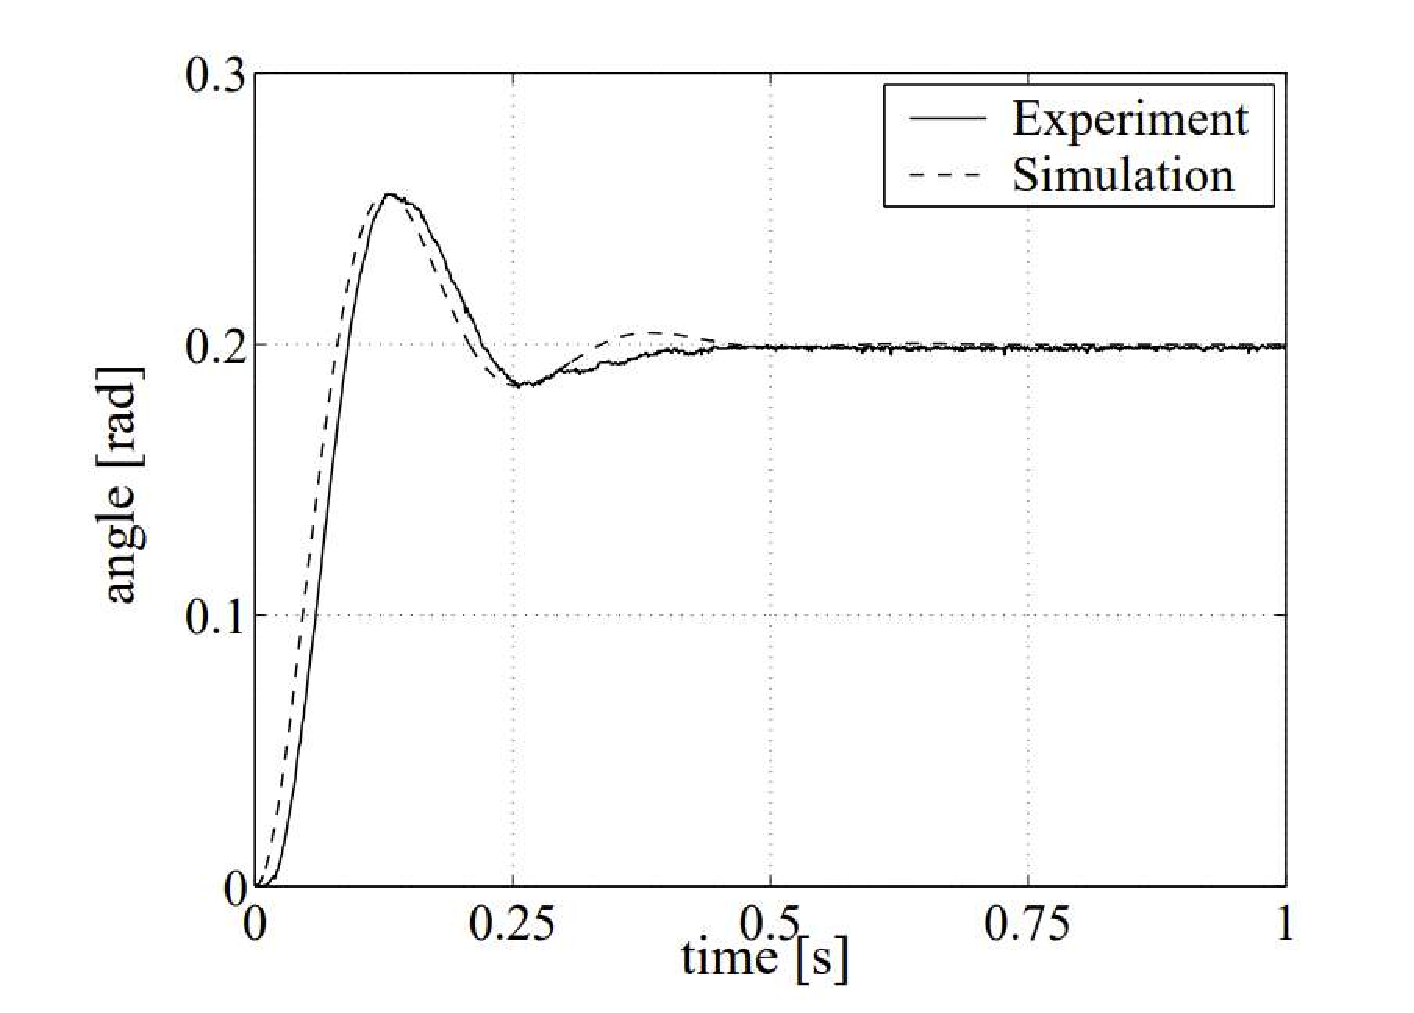
\includegraphics[width=\linewidth]{figure/thetax_response2.pdf}
        \caption{$\theta_x(t)$ の応答 ($\theta_x^{\mathrm{ref}}(t) = 0.2$, $\theta_y^{\mathrm{ref}}(t) = 0$)}
    \end{subfigure}
    \hfill
    \begin{subfigure}[b]{0.45\linewidth}
        \centering
        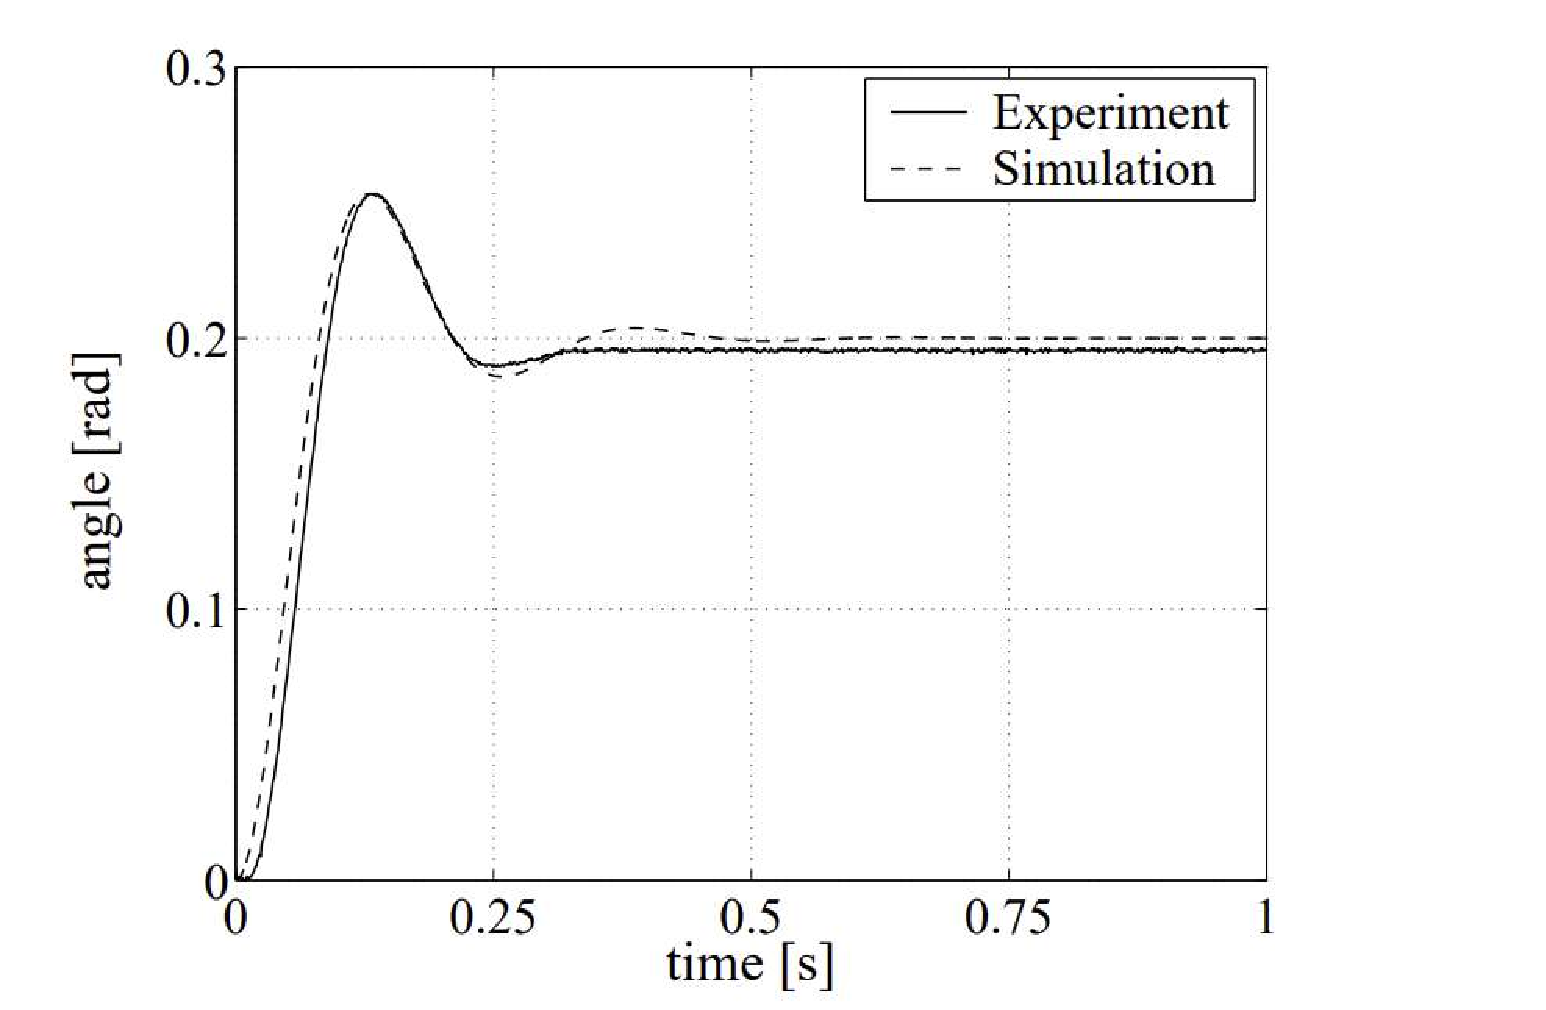
\includegraphics[width=\linewidth]{figure/thetay_response2.pdf}
        \caption{$\theta_y(t)$ の応答 ($\theta_x^{\mathrm{ref}}(t) = 0$, $\theta_y^{\mathrm{ref}}(t) = 0.2$)}
    \end{subfigure}
    \caption{P コントローラを用いたときのステップ応答 ($k_{Px}=20,\ k_{Py}=20$)}
    \label{fig:step_response2}
\end{figure}
